\section{Systemanforderungen}

Wir haben uns zuvor bei der Voranalyse mit den Problembereichen unseres Projekts befasst und die Haubtaufgaben extrahiert. Diese werden nun detaillierter beschrieben. 

\begin{figure}[htb]

	\centering

	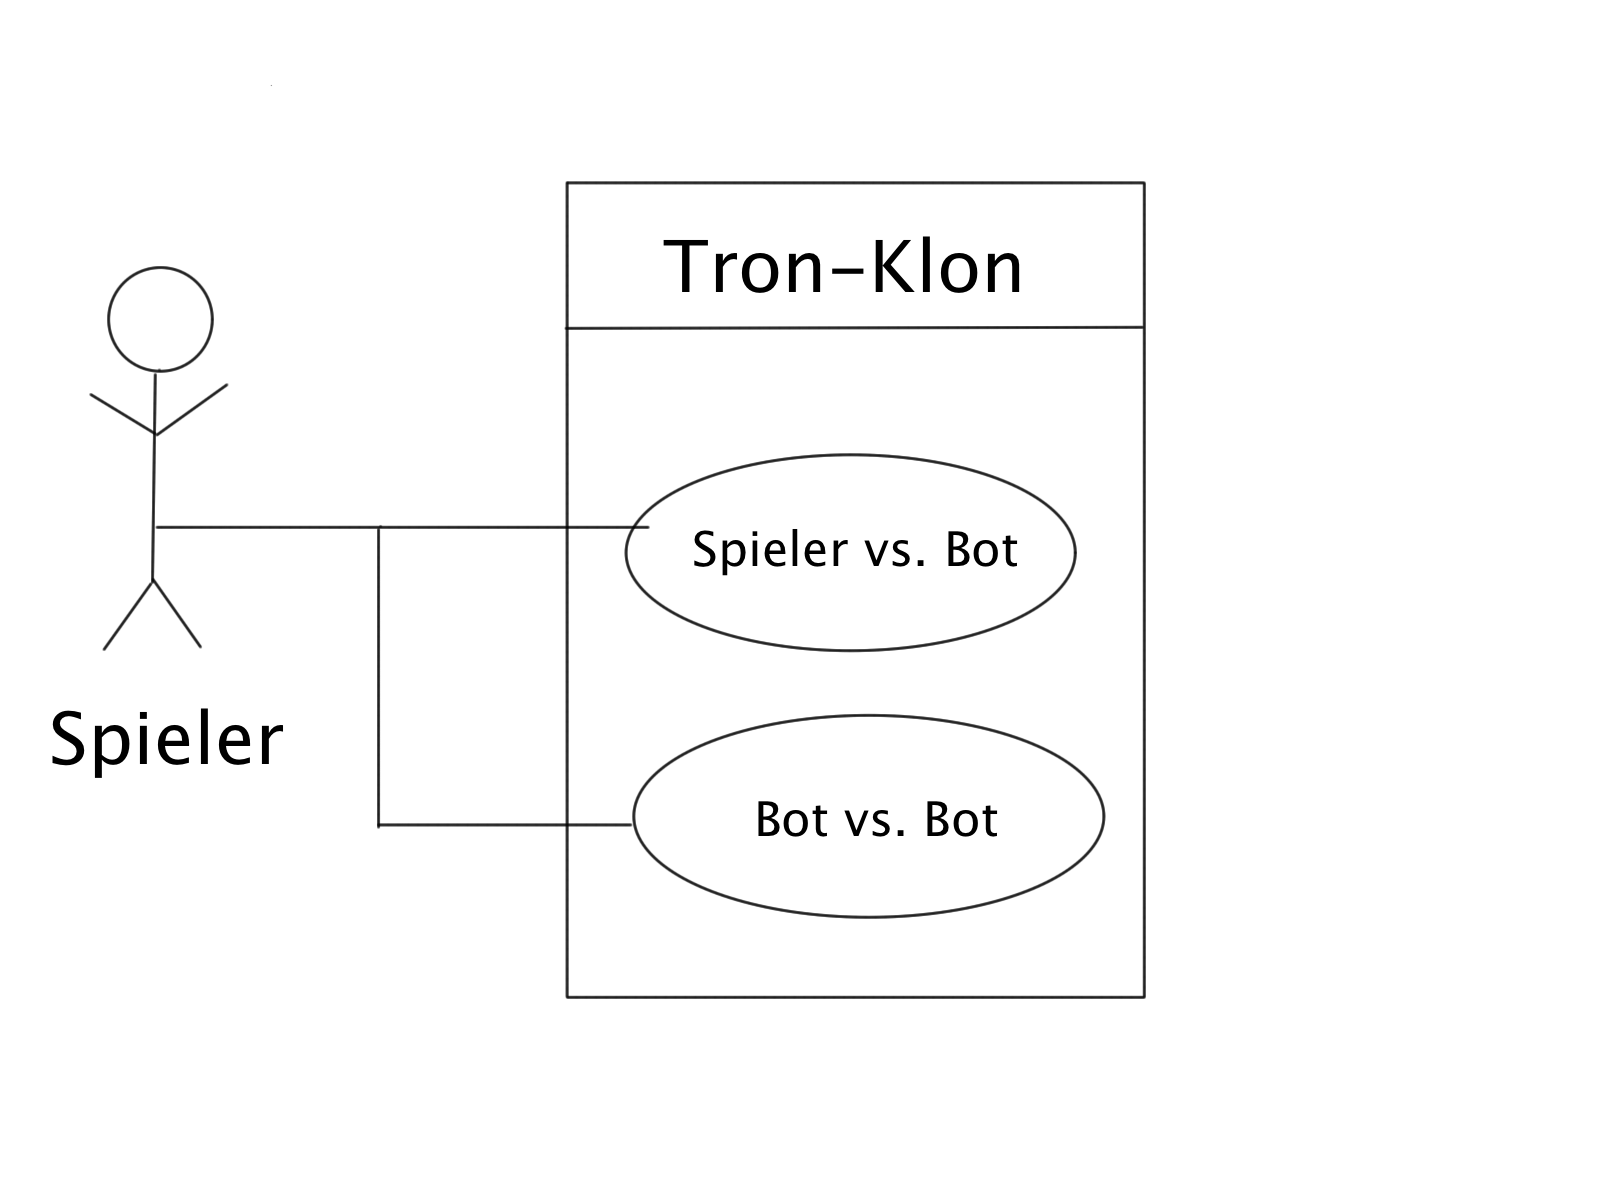
\includegraphics[width=7cm]{usecase.png}

	\caption{Übersicht Anwendungsfälle}

\end{figure}

\subsection{Übersicht Anwendungsfälle}

Bei unserem Projekt gibt es grundsätzlich zwei Anwendungsfälled. Zum einen die Möglichkeit auf dem eigenen System gegen die selbstlernenden Gegener (im folgenden Bots genannt) zu spielen oder einen Bot, der bereits trainiert wurde, zu exportieren und gegen einen Bot eines andern Spieler antreten zu lassen.

\subsection{Spieler gegen Bot}
\begin{tabularx}{\textwidth}{| X | X |}
	\hline
	Kurzbeschreibung & Ein Spieler tritt gegen einen oder mehrere Bots an und versucht gegen diese zu gewinnen. \\
	\hline
	Akteure & Bots und der Spieler. \\
	\hline
	Vorbedingungen & Der Spieler muss über das Proof of Concept verfügen. \\
	\hline
	Ablauf & Der Spieler startet ein neues Spiel.\\
	\hline
	Resultat & Das Spiel wird abgebrochen sobald nur noch der Spieler oder ein Bot am Leben ist. \\
	\hline
	Ausnahmen & In diesem Fall nicht möglich. \\
	\hline	
\end{tabularx}

\subsection{Bot gegen Bot}
\begin{tabularx}{\textwidth}{| X | X |}
	\hline
	Kurzbeschreibung & Zwei Bots treten gegeneinander an. Jeder von ihnen wurde auf einem unabhängigen System trainiert. \\
	\hline
	Akteure & Bot von Spieler Eins und Bot von Spieler Zwei. \\
	\hline
	Vorbedingungen & Beide Spieler müssen über das Proof of Concept verfügen. \\
	\hline
	Ablauf & Einer der beiden Spieler exportiert sein Bot und übergibt ihm dem anderen Spieler.\\
	\hline
	Resultat & Die beiden Bots spielen in erhöter Geschwindikeit bis einer gewinnt. \\
	\hline
	Ausnahmen & Die Übergabe des Bots fällt nicht in die Verantwortung des Proof of Concept.\\
	\hline
\end{tabularx}
\newpage
